\section{Vorbereitende Aufgaben}

\subsection{Die Quantenzahlen und die Landé-Faktoren von Cd-Atomen}

Die rote Spektrallinie von der Cd-Lampe entspricht dem Übergang ${^1P_1} \longleftrightarrow {^1D_2}$, die blaue Spektrallinie 
${^3S_1} \longleftrightarrow {^3P_1}$. Die zugehörige Quantenzahlen und die mit Formel \ref{eqn:gJ} berechneten Landé-Faktoren sind in Tabelle 
\ref{tab:v2} zu sehen. 
\FloatBarrier
\begin{table}
    \centering
    \caption{Quantenzahlen und Landé-Faktoren der verschiedenen Zustände.}
    \label{tab:v2}
    \sisetup{table-format=1.2}
    \begin{tabular}{c S[table-format=1.0] S[table-format=1.0] S[table-format=1.0] S[table-format=1.1] }
      \toprule
      %{$D$/cm}& \multicolumn{5}{c}{$U_{\symup{B}i} = \,\si{V}$}\\ überschrift über mehrere spalten
      %\midrule
       {Zustand} & {$L$}& {$S$} & {$J$} & {$g_{\si{j}}$}\\
      \midrule
      \midrule
        {${^1P_1}$} & 1 & 0 & 1 & 1\\ 
        {${^1D_2}$} & 2 & 0 & 2 & 1\\ 
        {${^3S_1}$} & 0 & 1 & 1 & 2\\ 
        {${^3P_1}$} & 1 & 1 & 1 & $\frac{3}{2}$\\ 
      \bottomrule
    \end{tabular}
\end{table}
\FloatBarrier

\subsection{Dispersionsgebiet und spektrale Auflösung des Messapperatur}
Mit Formel \ref{eqn:lD} und \ref{eqn:A} wird das Dispersionsgebiet $\lambda_{\si{D}}$ und das 
Auflösungsvermögen $A$ für die rote und die blaue Spektrallinie berechnet, was in Tabelle \ref{tab:v1} 
eingetragen ist. 
Die dafür benötigten Werte 
\begin{align*}
  \lambda_{\si{rot}} &= \SI{643.8}{\nano\meter},\\
  \lambda_{\si{blau}}&= \SI{480}{\nano\meter}, \\
  d &= \SI{4}{\milli\meter},\\
  L &=\SI{120}{\milli\meter},\\
  n_{\si{rot}} &=\num{1.4567},\\
  n_{\si{blau}} &= \num{1.4635}\\
\end{align*}
werden der Versuchsanleitung [1] entnommen. 

\FloatBarrier
\begin{table}
    \centering
    \caption{Dispersionsgebiet und Auflösungsvermögen der Lummer-Gehrcke-Platte.}
    \label{tab:v1}
    \sisetup{table-format=1.2}
    \begin{tabular}{c S[table-format=2.1] S[table-format=6.0] }
      \toprule
      %{$D$/cm}& \multicolumn{5}{c}{$U_{\symup{B}i} = \,\si{V}$}\\ überschrift über mehrere spalten
      %\midrule
       {Spektrallinie} & {$\lambda_{\si{D}}/\si{pm}$}& {$A$}\\
      \midrule
      \midrule
        rot & 48,9 & 209129 \\
        blau & 27,0 & 285458 \\
      \bottomrule
    \end{tabular}
\end{table}
\FloatBarrier


\subsection{Optimale Einstellung der Magnetfeldstärke}

Die optimale Einstellung der Magnetfeldstärke berechnet sich durch die Formel 
\begin{equation*}
  B_{\si{optim}}= \frac{1}{4} \lambda_{\si{D}} \frac{h c}{\lambda² (m_i g_{Ji} - m_j g_{Jj}) \mu_B}.
\end{equation*}
Für die beiden Linien sind die optimalen Magnetfelder in Tabelle \ref{tab:A} zusammengefasst. Die rote 
hat für $m_i g_{Ji} - m_j g_{Jj}$ immer nur den Wert 1, für die blaue Linie werden zwei verschiedne Übergänge 
beobachtet, ein mal mit $m_i g_{Ji} - m_j g_{Jj} = 2$ und $m_i g_{Ji} - m_j g_{Jj} = \frac{1}{2}$.

\begin{table}
    \centering
    \caption{Optimale Magentfelder.}
    \label{tab:A}
    \sisetup{table-format=1.2}
    \begin{tabular}{c S[table-format=2.1] S[table-format=6.0] S S}
      \toprule
      %{$D$/cm}& \multicolumn{5}{c}{$U_{\symup{B}i} = \,\si{V}$}\\ überschrift über mehrere spalten
      %\midrule
       {Spektrallinie} & {$\lambda$}/nm &{$\lambda_{\si{D}}/\si{pm}$}& {$m_i g_{Ji} - m_j g_{Jj}$} & {$B_{\si{optim}}$/T}\\
      \midrule
      \midrule
        rot  & 643,8  &  48,9 & 1   & 0,62\\
        blau & 480    &  27,0 & 2   & 0,31\\
        blau & 480    &  27,0 & 0,5 & 1,25\\
      \bottomrule
    \end{tabular}
\end{table}
\FloatBarrier




\section{Auswertung}
\label{sec:Auswertung}

%\subsection{Einführung}


%\FloatBarrier

%Einheiten: \SI{3}{\newton\s}
%1,41 \cdot \cramped{10^{-3}} ~s  für hochzahlen

%\begin{table}
%  \centering
%  \caption{Tabelle für a)Erste Bestimmung der Zeitkonstanten}
%  \label{Tab1}
%    \begin{tabular}{c c}%c zeigt die anzahl der Spalten
%      \toprule
%      Spannung $U_c$ &Zeit $t$\\% \\ werden benötigt um die Zeile zu Beenden
%      mV&ms\\% & Zeichen grenzen die Zahlen voneinander ab.
%      \midrule
%      \midrule
%        %\input{tab1.txt}% Die Tabelle ist hier ausgelagert. Sie kann aber auch genausogut hier eingefügt werden.
%          0,000 &     752\\
%          0,400 &     440\\
%          0,800 &     448\\
%      \bottomrule
%    \end{tabular}
%\end{table}

%Mittelwert von X:
%\begin{equation*}
%  \overline{X }=  \frac{1}{N} \sum_{i=1}^N (X_i) = 75,98 \, \si{Hz} 
%\end{equation*}
%Formel für den Fehler des Mittelwerts:
%\begin{equation*}
%  \symup{\Delta} X = \frac{1}{\sqrt{N}} \sqrt{\frac{1}{\sqrt{N-1}} \sum_{i=1}^N (X_{i}-\overline{X})²}= 0,02 \, \si{Hz} 
%\end{equation*}


\subsection{Bestimmung des Magnetfeldes}
Zur Bestimmung der Magnetfeldstärke wird bei verschiedenen Stromstärken $I$ die magnetische Feldstärke $B$ mit einer Hall-Sonde
gemessen. Die damei ermittelten Werte sind in Tabelle \ref{tab:a} eingetragen.
\FloatBarrier
\begin{table}
    \centering
    \caption{Magnetfeldstärke in Abhängigkeit von der Stromstärke.}
    \label{tab:a}
    \sisetup{table-format=1.2}
    \begin{tabular}{S[table-format=1.1] S[table-format=1.3] S[table-format=1.1] S[table-format=1.3] }
      \toprule
      %{$D$/cm}& \multicolumn{5}{c}{$U_{\symup{B}i} = \,\si{V}$}\\ überschrift über mehrere spalten
      %\midrule
       {$I/\si{A}$}& {$B/\si{T}$} & {$I/\si{A}$}& {$B/\si{T}$}\\
      \midrule
      \midrule
      1,0 & 0,138 & 4,0 & 0,621 \\ 
      1,4 & 0,205 & 4,2 & 0,663 \\
      1,8 & 0,278 & 4,4 & 0,688 \\
      2,0 & 0,308 & 4,8 & 0,815 \\
      2,2 & 0,335 & 5,0 & 0,862 \\
      2,4 & 0,362 & 5,2 & 0,885 \\
      2,8 & 0,421 & 5,4 & 0,970 \\
      3,2 & 0,484 & 5,6 & 1,064 \\
      3,6 & 0,544 & 5,8 & 1,108 \\
      3,8 & 0,585 & 6,0 & 1,155 \\
      \bottomrule
    \end{tabular}
\end{table}
\FloatBarrier
Hierzu wird eine lineare Regression 
\begin{equation}
    \label{eqn:B}
    B = a \cdot I + b
\end{equation} durchgeführt. Diese ist in Abbildung \ref{fig:a} dargestellt.
\FloatBarrier
\begin{figure}
  \centering
  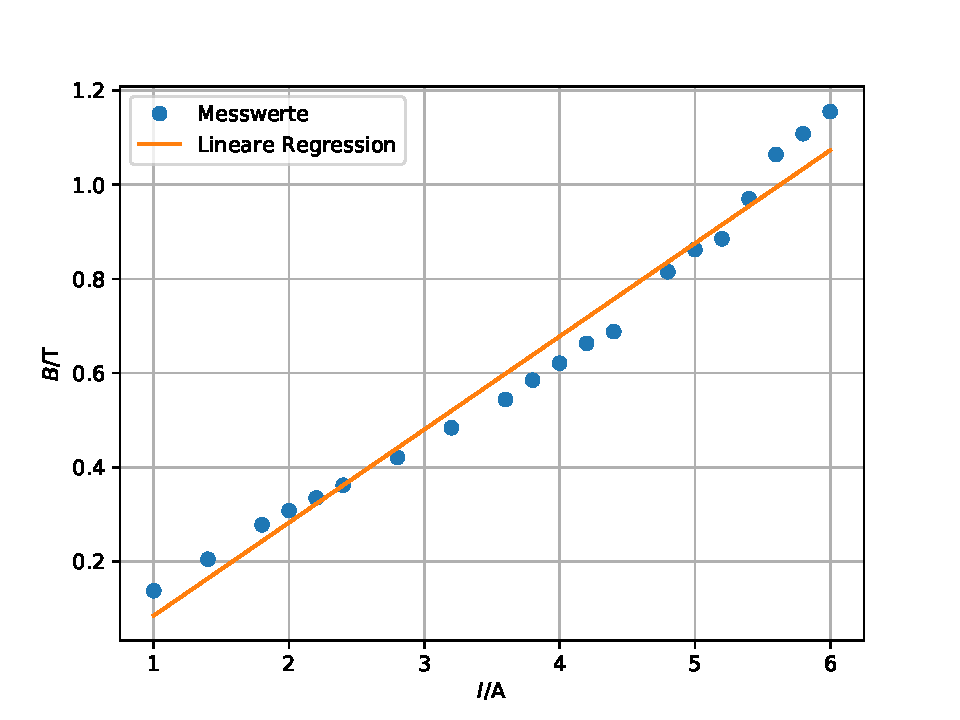
\includegraphics[width=0.8\textwidth]{a.pdf}
  \caption{Magnetfeldstärke in Abhängigkeit von der Stromstärke mit linearer Regression.}
  \label{fig:a}
\end{figure}
\FloatBarrier
Es ergeben sich die Werte 
\begin{align*}
    a &= \SI{0.198\pm0.007}{\tesla\per\ampere} \\
    b &= \SI{-0.112\pm0.029}{\tesla}.
\end{align*}

\subsection{Bestimmung der Wellenlängenverschiebung}
\subsubsection{Rote Spektrallinie}
Zunächst wird das Interferenzmuster für rotes Licht untersucht. 
Hierbei wird ein Strom von $I=\SI{4.0}{\ampere}$ eingestellt, was nach Formel \ref{eqn:B} einem Magnetfeld von 
\begin{equation*}
    B_{\si{rot}} = \SI{0.678\pm0.040}{\tesla} 
\end{equation*}
entspricht.
In Abbildung \ref{fig:r1} ist das Interferenzbild ohne Magnetfeld zu sehen. Dieses wurde nachträglich aufgehellt, um die Abstände zwischen den Maxima besser 
sehen zu können.

\FloatBarrier
\begin{figure}
  \centering
  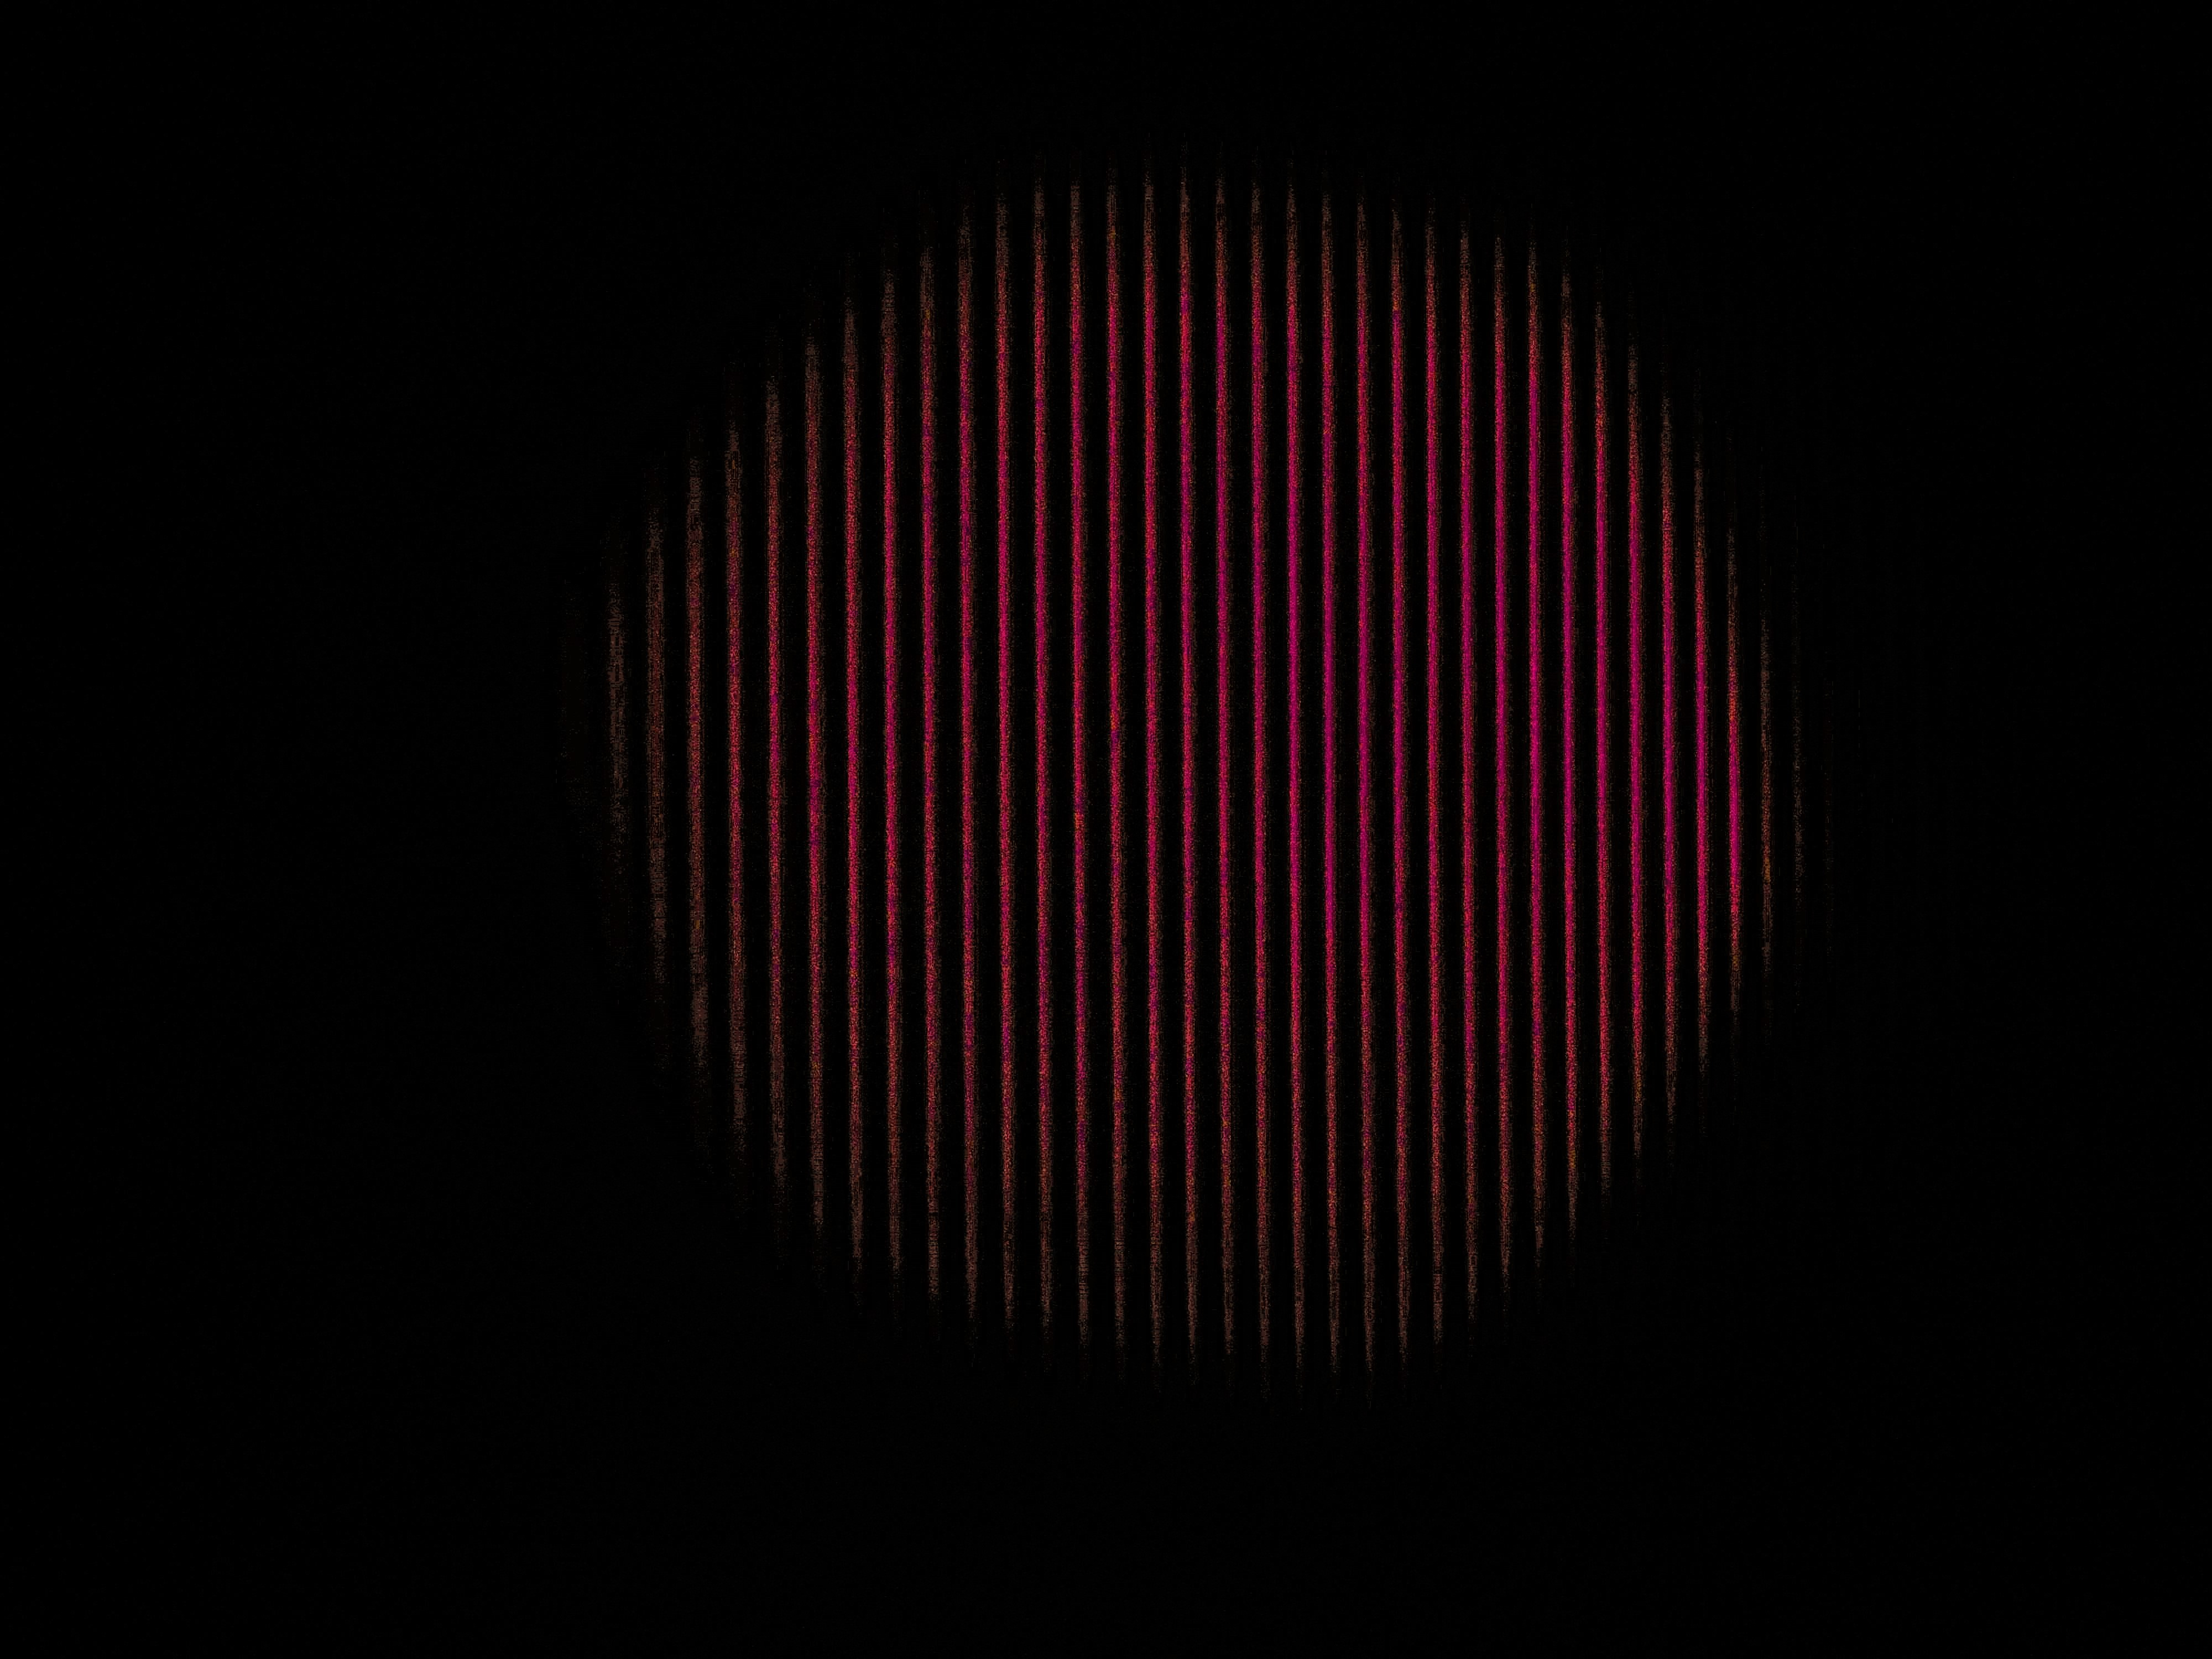
\includegraphics[width=0.45\textwidth]{IMG_0103k.jpg}
  \caption{Interferenzmuster der roten Spektrallinie ohne Magnetfeld (nachbearbeitet).}
  \label{fig:r1}
\end{figure}
\FloatBarrier

Nachfolgend sind die Interferenzmuster bei einem Polarisationsfilter, der nur linear polarisiertes Licht durchlässt (\ref{fig:r2}), und einem für zirkular polarisiertes Licht (\ref{fig:r3}) 
bei eingeschaltetem Magnetfeld dargestellt. Auch diese Bilder wurden nachträglich bearbeitet.

\FloatBarrier
\begin{figure}
  \centering
  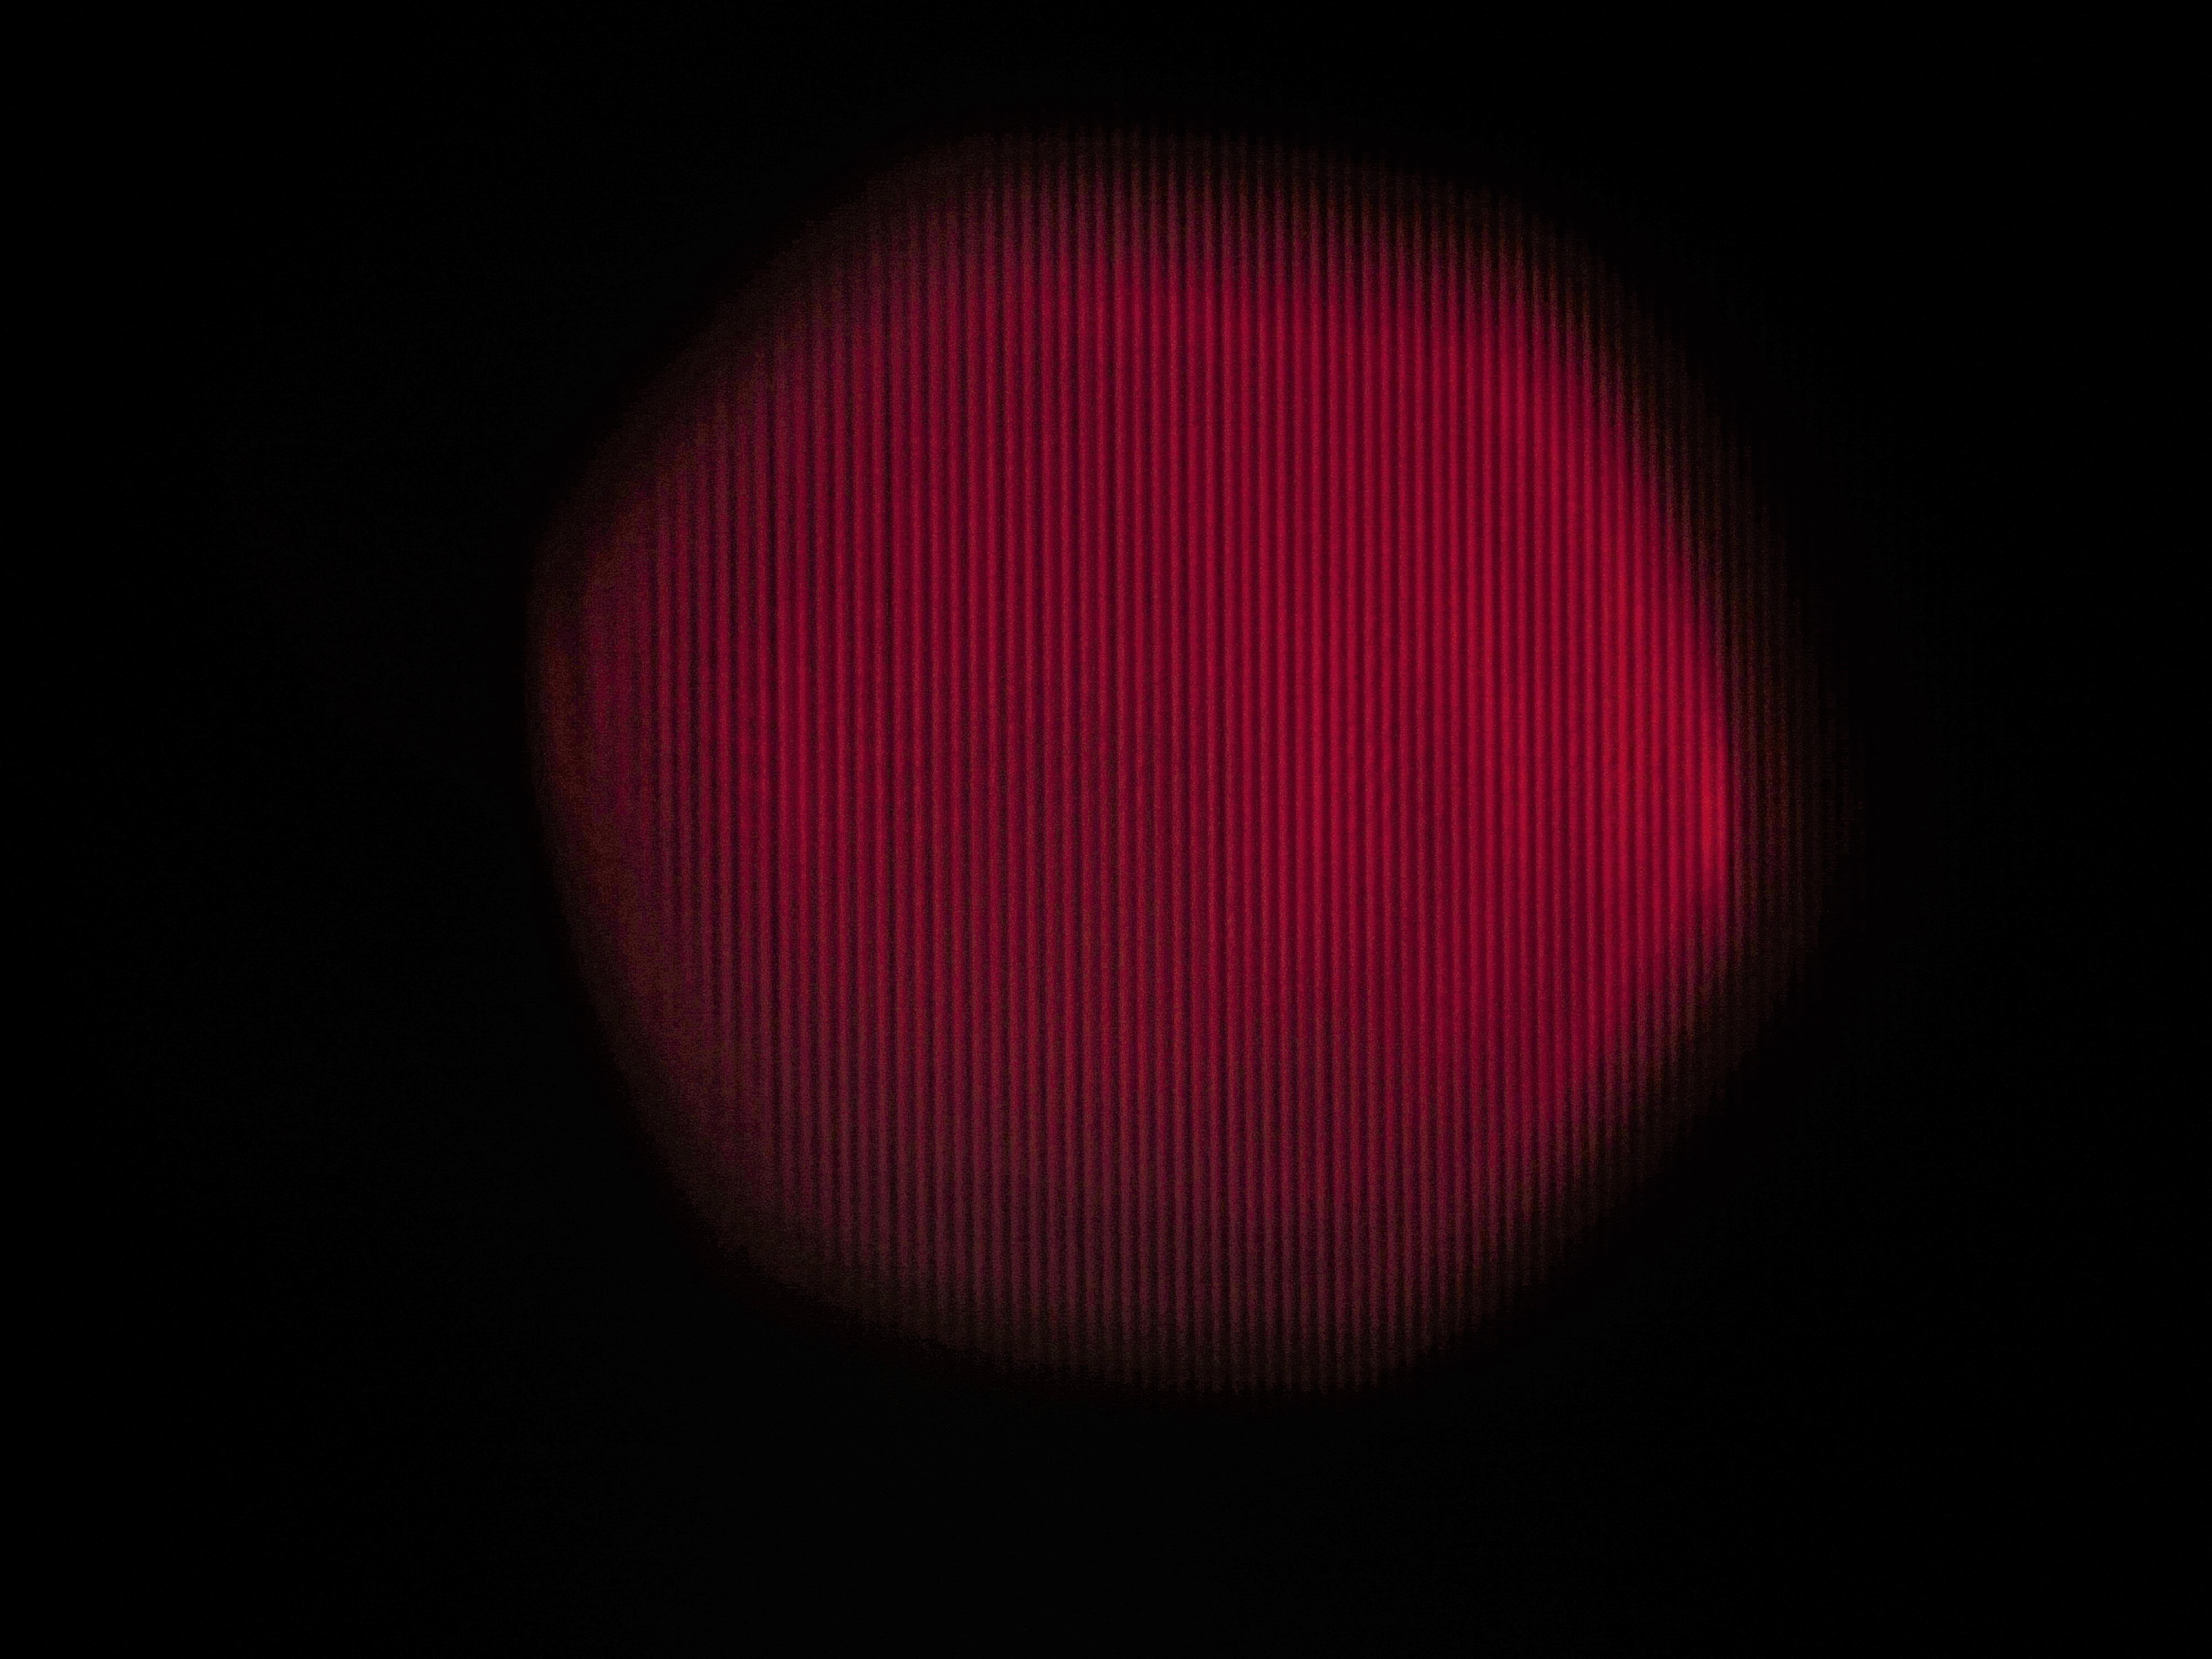
\includegraphics[width=0.45\textwidth]{IMG_0104k.jpg}
  \caption{Interferenzmuster der roten Spektrallinie mit linear polarisiertem Licht mit Magnetfeld (nachbearbeitet).}
  \label{fig:r2}
\end{figure}
\FloatBarrier
\FloatBarrier
\begin{figure}
  \centering
  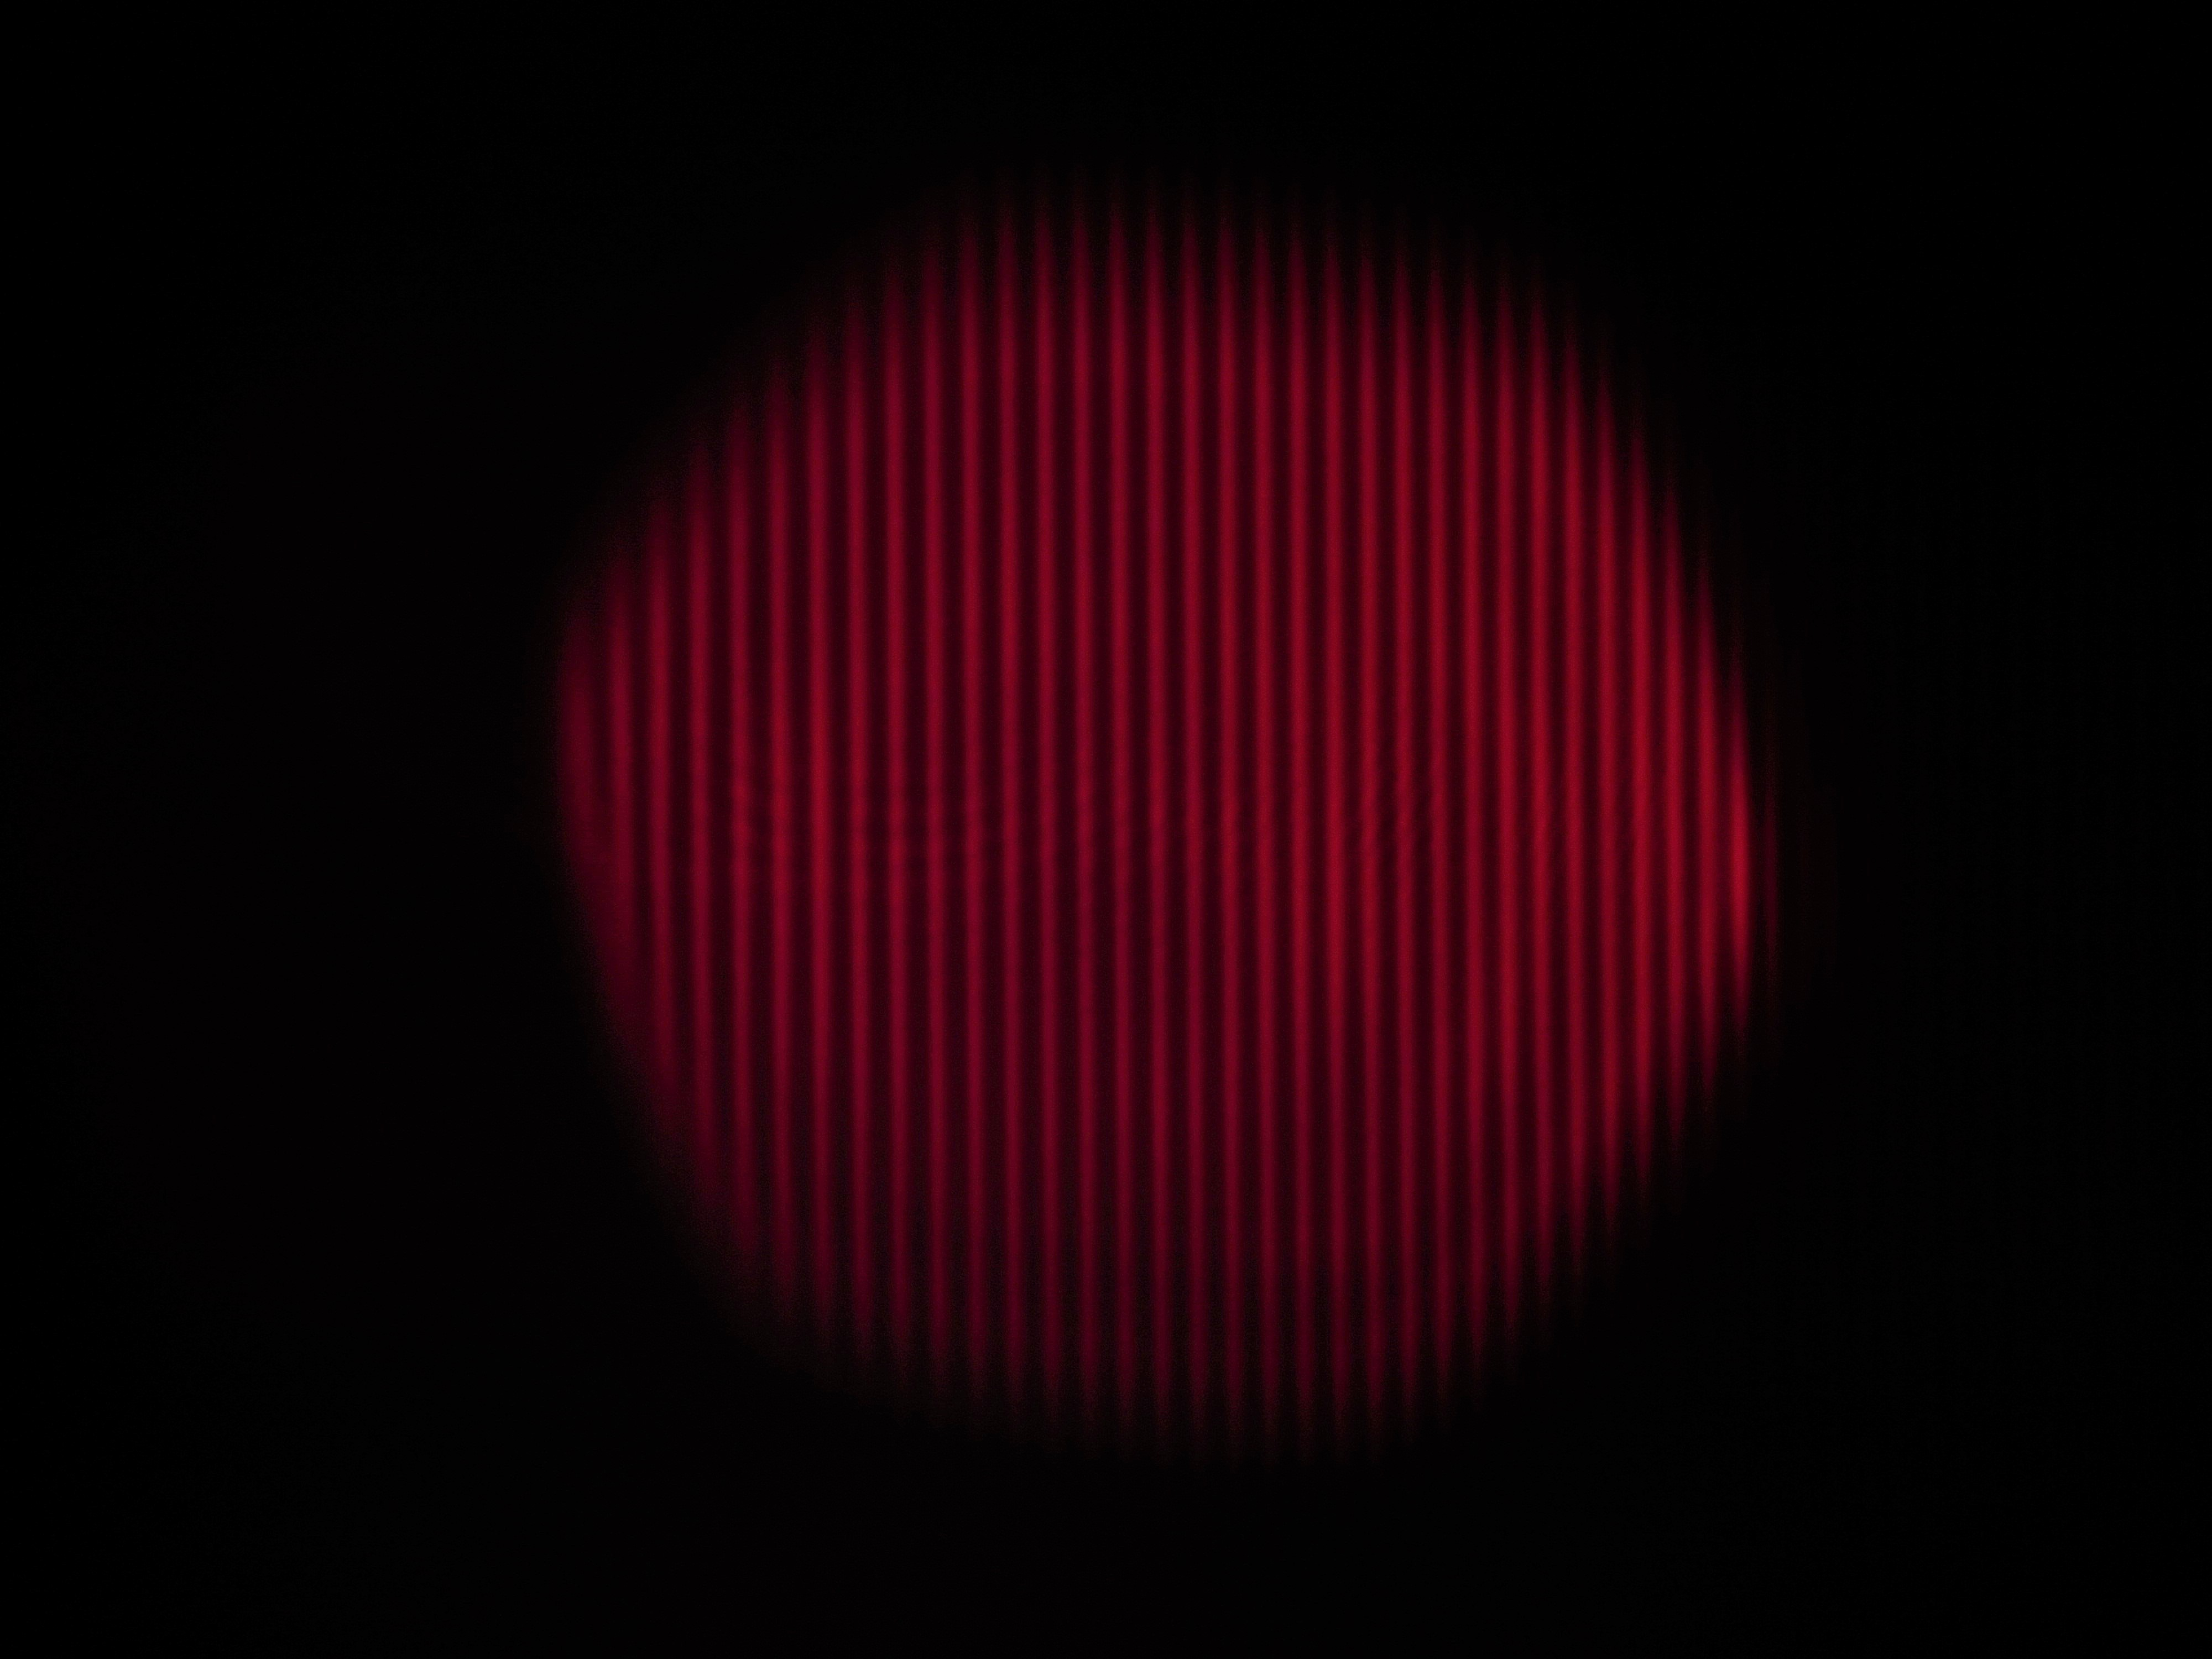
\includegraphics[width=0.45\textwidth]{IMG_0105k.jpg}
  \caption{Interferenzmuster der roten Spektrallinie mit zirkular polarisiertem Licht mit Magnetfeld (nachbearbeitet).}
  \label{fig:r3}
\end{figure}
\FloatBarrier

Die gemessenen Abstände $\increment s$ und  $\delta s$ sowie die mit Formel
\ref{eqn:} % fehlt noch
Wellenlängenunterschiede $\increment \lambda$ sind in Tabelle \ref{tab:r} eingetragen. Da sich bei Abbildung \ref{fig:r3}
nichts im Vergleich zu Abbildung \ref{fig:r1} geändert hat, werden die Werte auch nicht berücksichtigt. 

\FloatBarrier
\begin{table}
    \centering
    \caption{Magnetfeldstärke in Abhängigkeit von der Stromstärke.}
    \label{tab:a}
    \sisetup{table-format=1.2}
    \begin{tabular}{S[table-format=3.0] S[table-format=3.0] S[table-format=2.2] }
      \toprule
      %{$D$/cm}& \multicolumn{5}{c}{$U_{\symup{B}i} = \,\si{V}$}\\ überschrift über mehrere spalten
      %\midrule
      {$\increment s_{\si{r}}/\text{Pixel}$} & {$\delta s_{\text{r,\,}\sigma}\text{Pixel}$} & {$\increment \lambda/\text{pm}$}\\
      \midrule
      \midrule
      68 & 39 & 14,02 \\
      70 & 33 & 11,53 \\
      74 & 34 & 11,23 \\
      68 & 35 & 12,58 \\
      74 & 36 & 11,89 \\
      72 & 33 & 11,21 \\
      66 & 32 & 11,85 \\
      70 & 36 & 12,57 \\
      72 & 31 & 10,53 \\
      62 & 33 & 13,01 \\
      72 & 36 & 12,23 \\
      66 & 35 & 12,97 \\
      64 & 31 & 11,84 \\
      70 & 33 & 11,53 \\
      62 & 29 & 11,44 \\
      64 & 29 & 11,08 \\
      64 & 27 & 10,31 \\
      64 & 30 & 11,46 \\
      62 & 29 & 11,44 \\
      64 & 26 &  9,33 \\
      62 & 34 & 13,41 \\
      64 & 33 & 12,61 \\
      62 & 31 & 12,23 \\
      69 & 30 & 10,63 \\
      63 & 37 & 14,36 \\
      59 & 34 & 14,09 \\
      61 & 28 & 11,22 \\
      61 & 34 & 13,63 \\
      59 & 29 & 12,02 \\
      61 & 31 & 12,43 \\
      58 & 29 & 12,23 \\
      \bottomrule
    \end{tabular}
\end{table}
\FloatBarrier

Gemittelt mit der Formel des Mittelwert 
\begin{equation}
  \label{eqn:X}
  \overline{X} = \frac{1}{N} \sum_{i=1}^N (X_i)
\end{equation}
und der für den Fehler des Mittelwerts 
\begin{equation}
    \label{eqn:dX}
    \symup{\Delta} X = \frac{1}{\sqrt{N}} \sqrt{\frac{1}{\sqrt{N-1}} \sum_{i=1}^N (X_{i}-\overline{X})²}
\end{equation}
ist die Wellenlängenverschiebung 
\begin{equation*}
  \increment \lambda = \SI{12.05\pm0.20}{\pico\meter}.
\end{equation*}

\subsubsection{Blaue Specktrallinie}
Bei der blauen Spektrallinie wird für die $\pi$-Linie ein Strom von $I_{\text{b,\,}\sigma} = \SI{2.0}{\ampere}$ und für die $\pi$-Linie $I_{\text{b,\,}\pi} = \SI{5.2}{\ampere}$ eingestellt. 
Das entspricht nach Formel \ref{eqn:B} einer Magnetfeldstärke  von 
\begin{align*}
 B_{\text{b,\,}\sigma} &= \SI{0.283}{\tesla},\\
 B_{\text{b,\,}\pi} &=\SI{0.915}{\tesla}.
\end{align*} 
Die zugehörigen Interferenzbilder sind in Abbildung \ref{fig:b1}, \ref{fig:b2} und \ref{fig:b3} zu sehen. 
\FloatBarrier
\begin{figure}
  \centering
  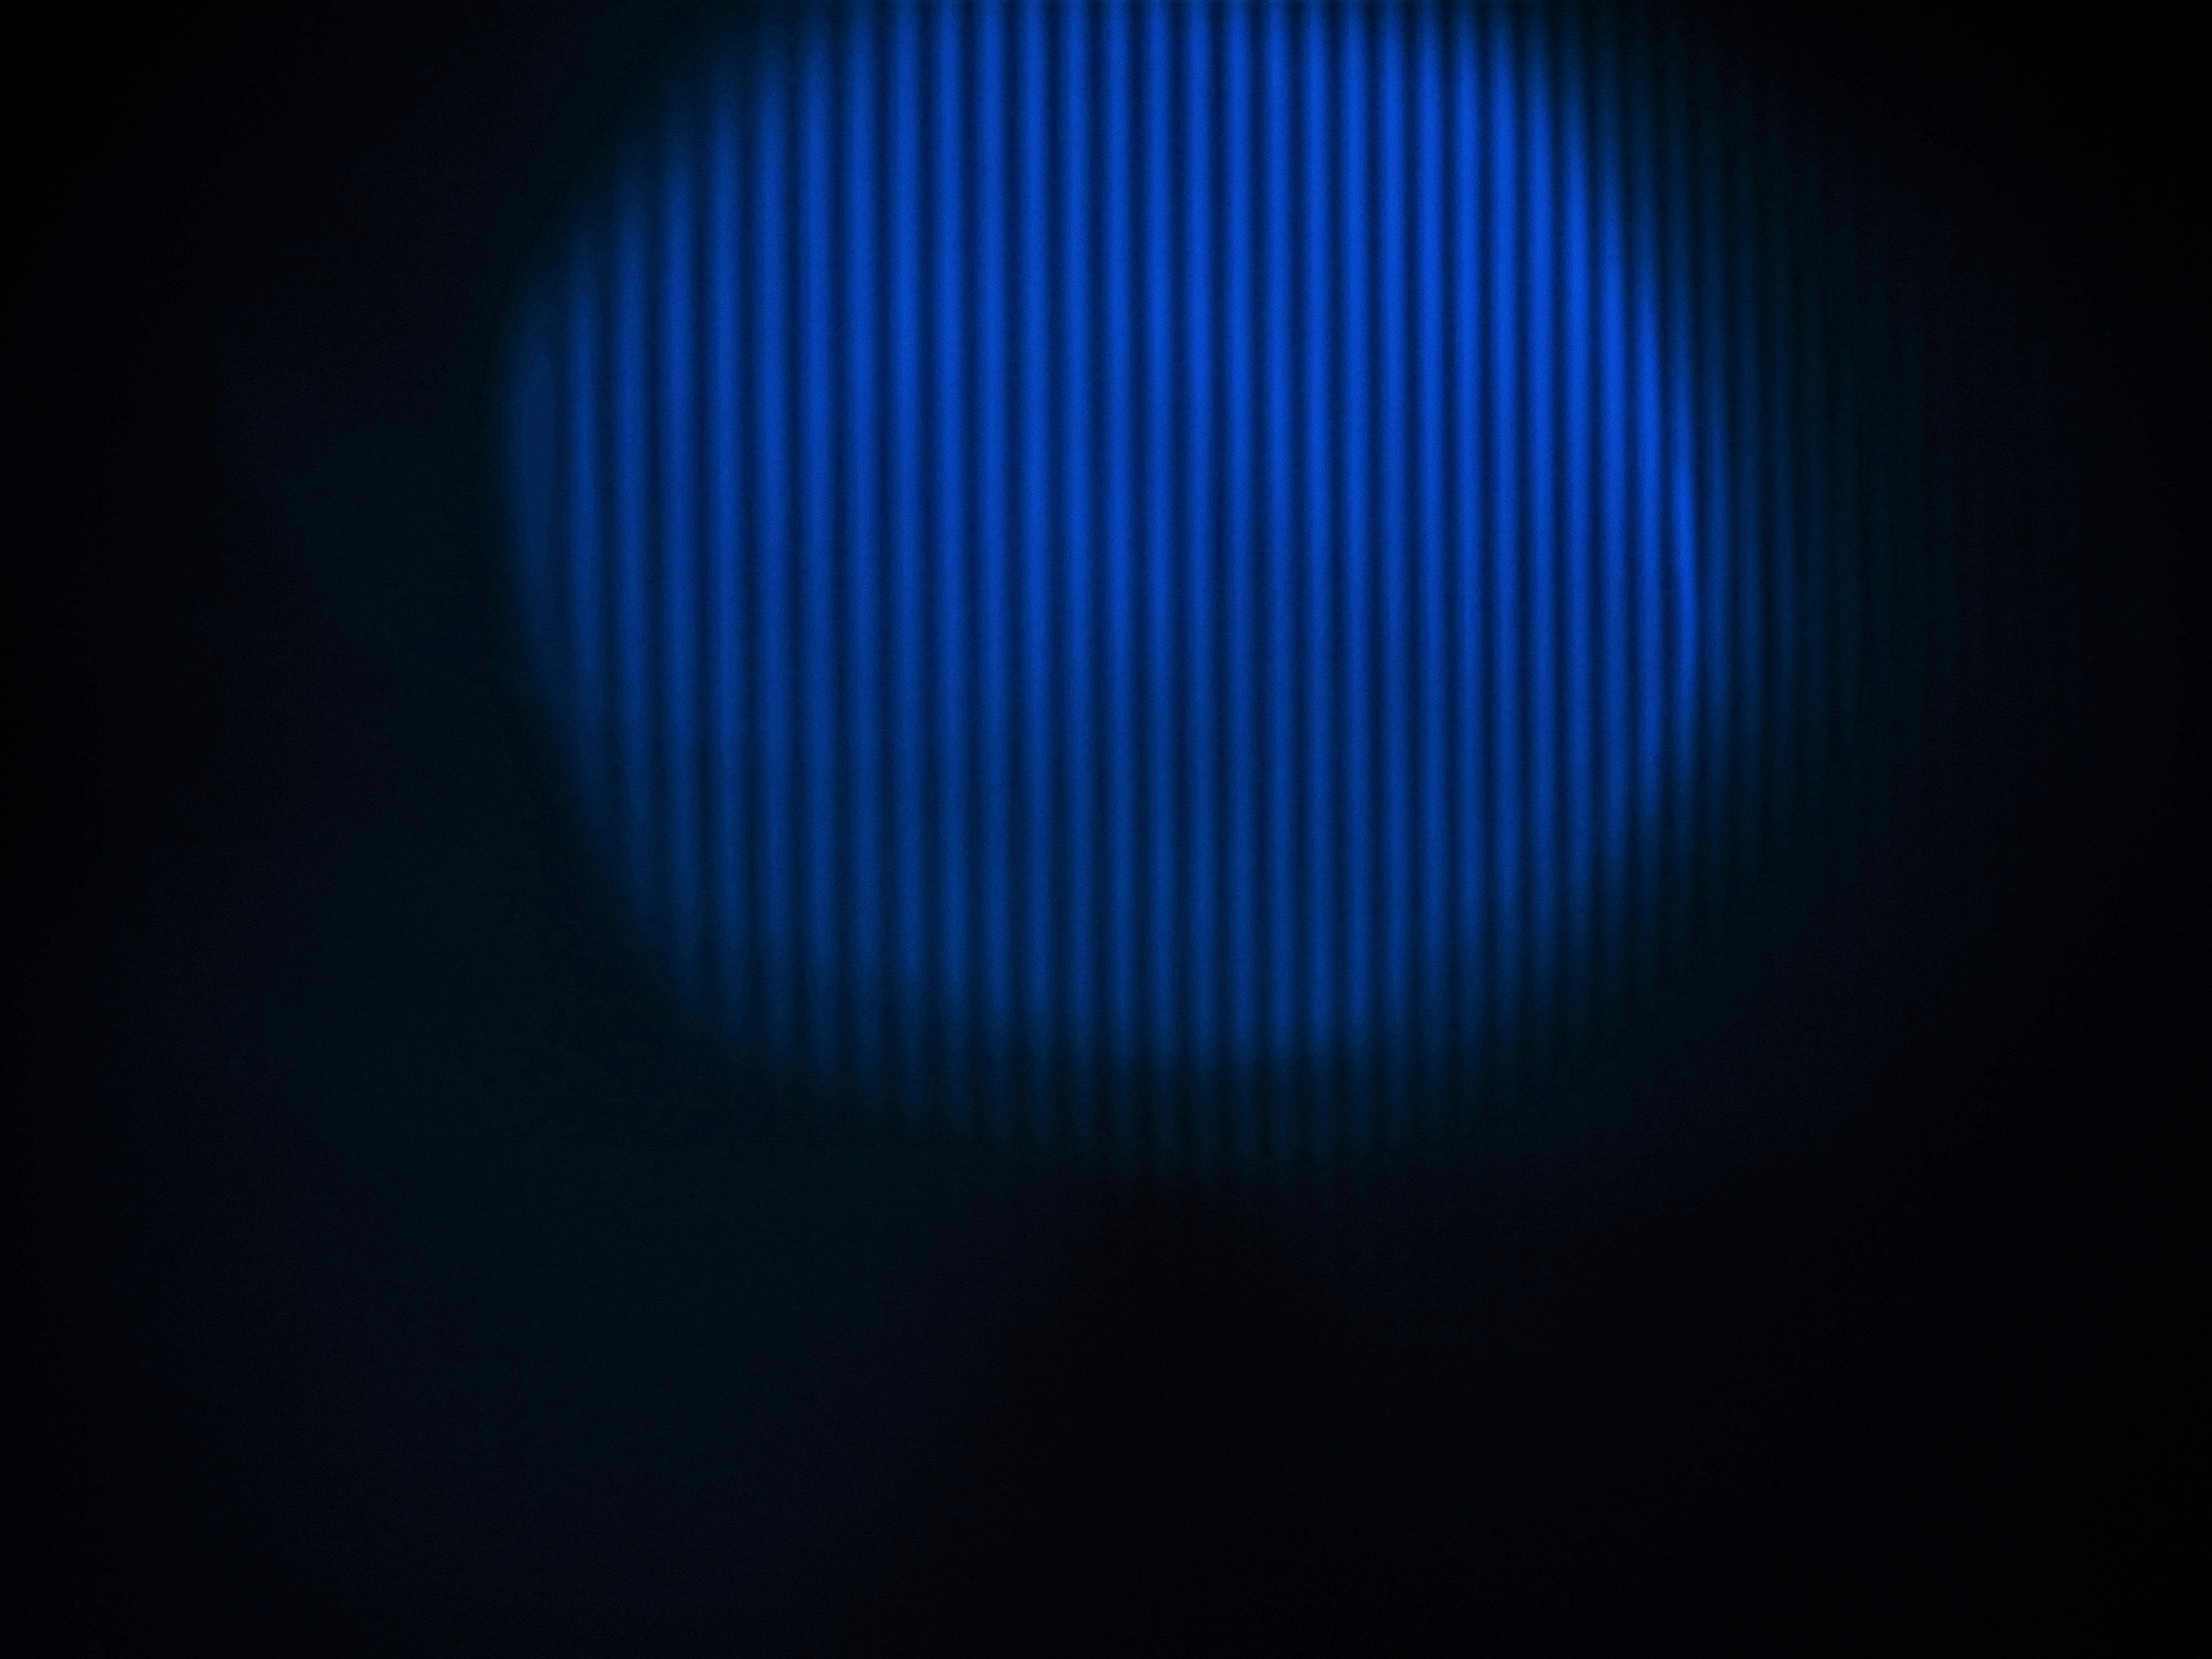
\includegraphics[width=0.45\textwidth]{IMG_0121k.jpg}
  \caption{Interferenzmuster der blauen Spektrallinie ohne Magnetfeld (nachbearbeitet).}
  \label{fig:b1}
\end{figure}
\FloatBarrier
\begin{figure}
  \centering
  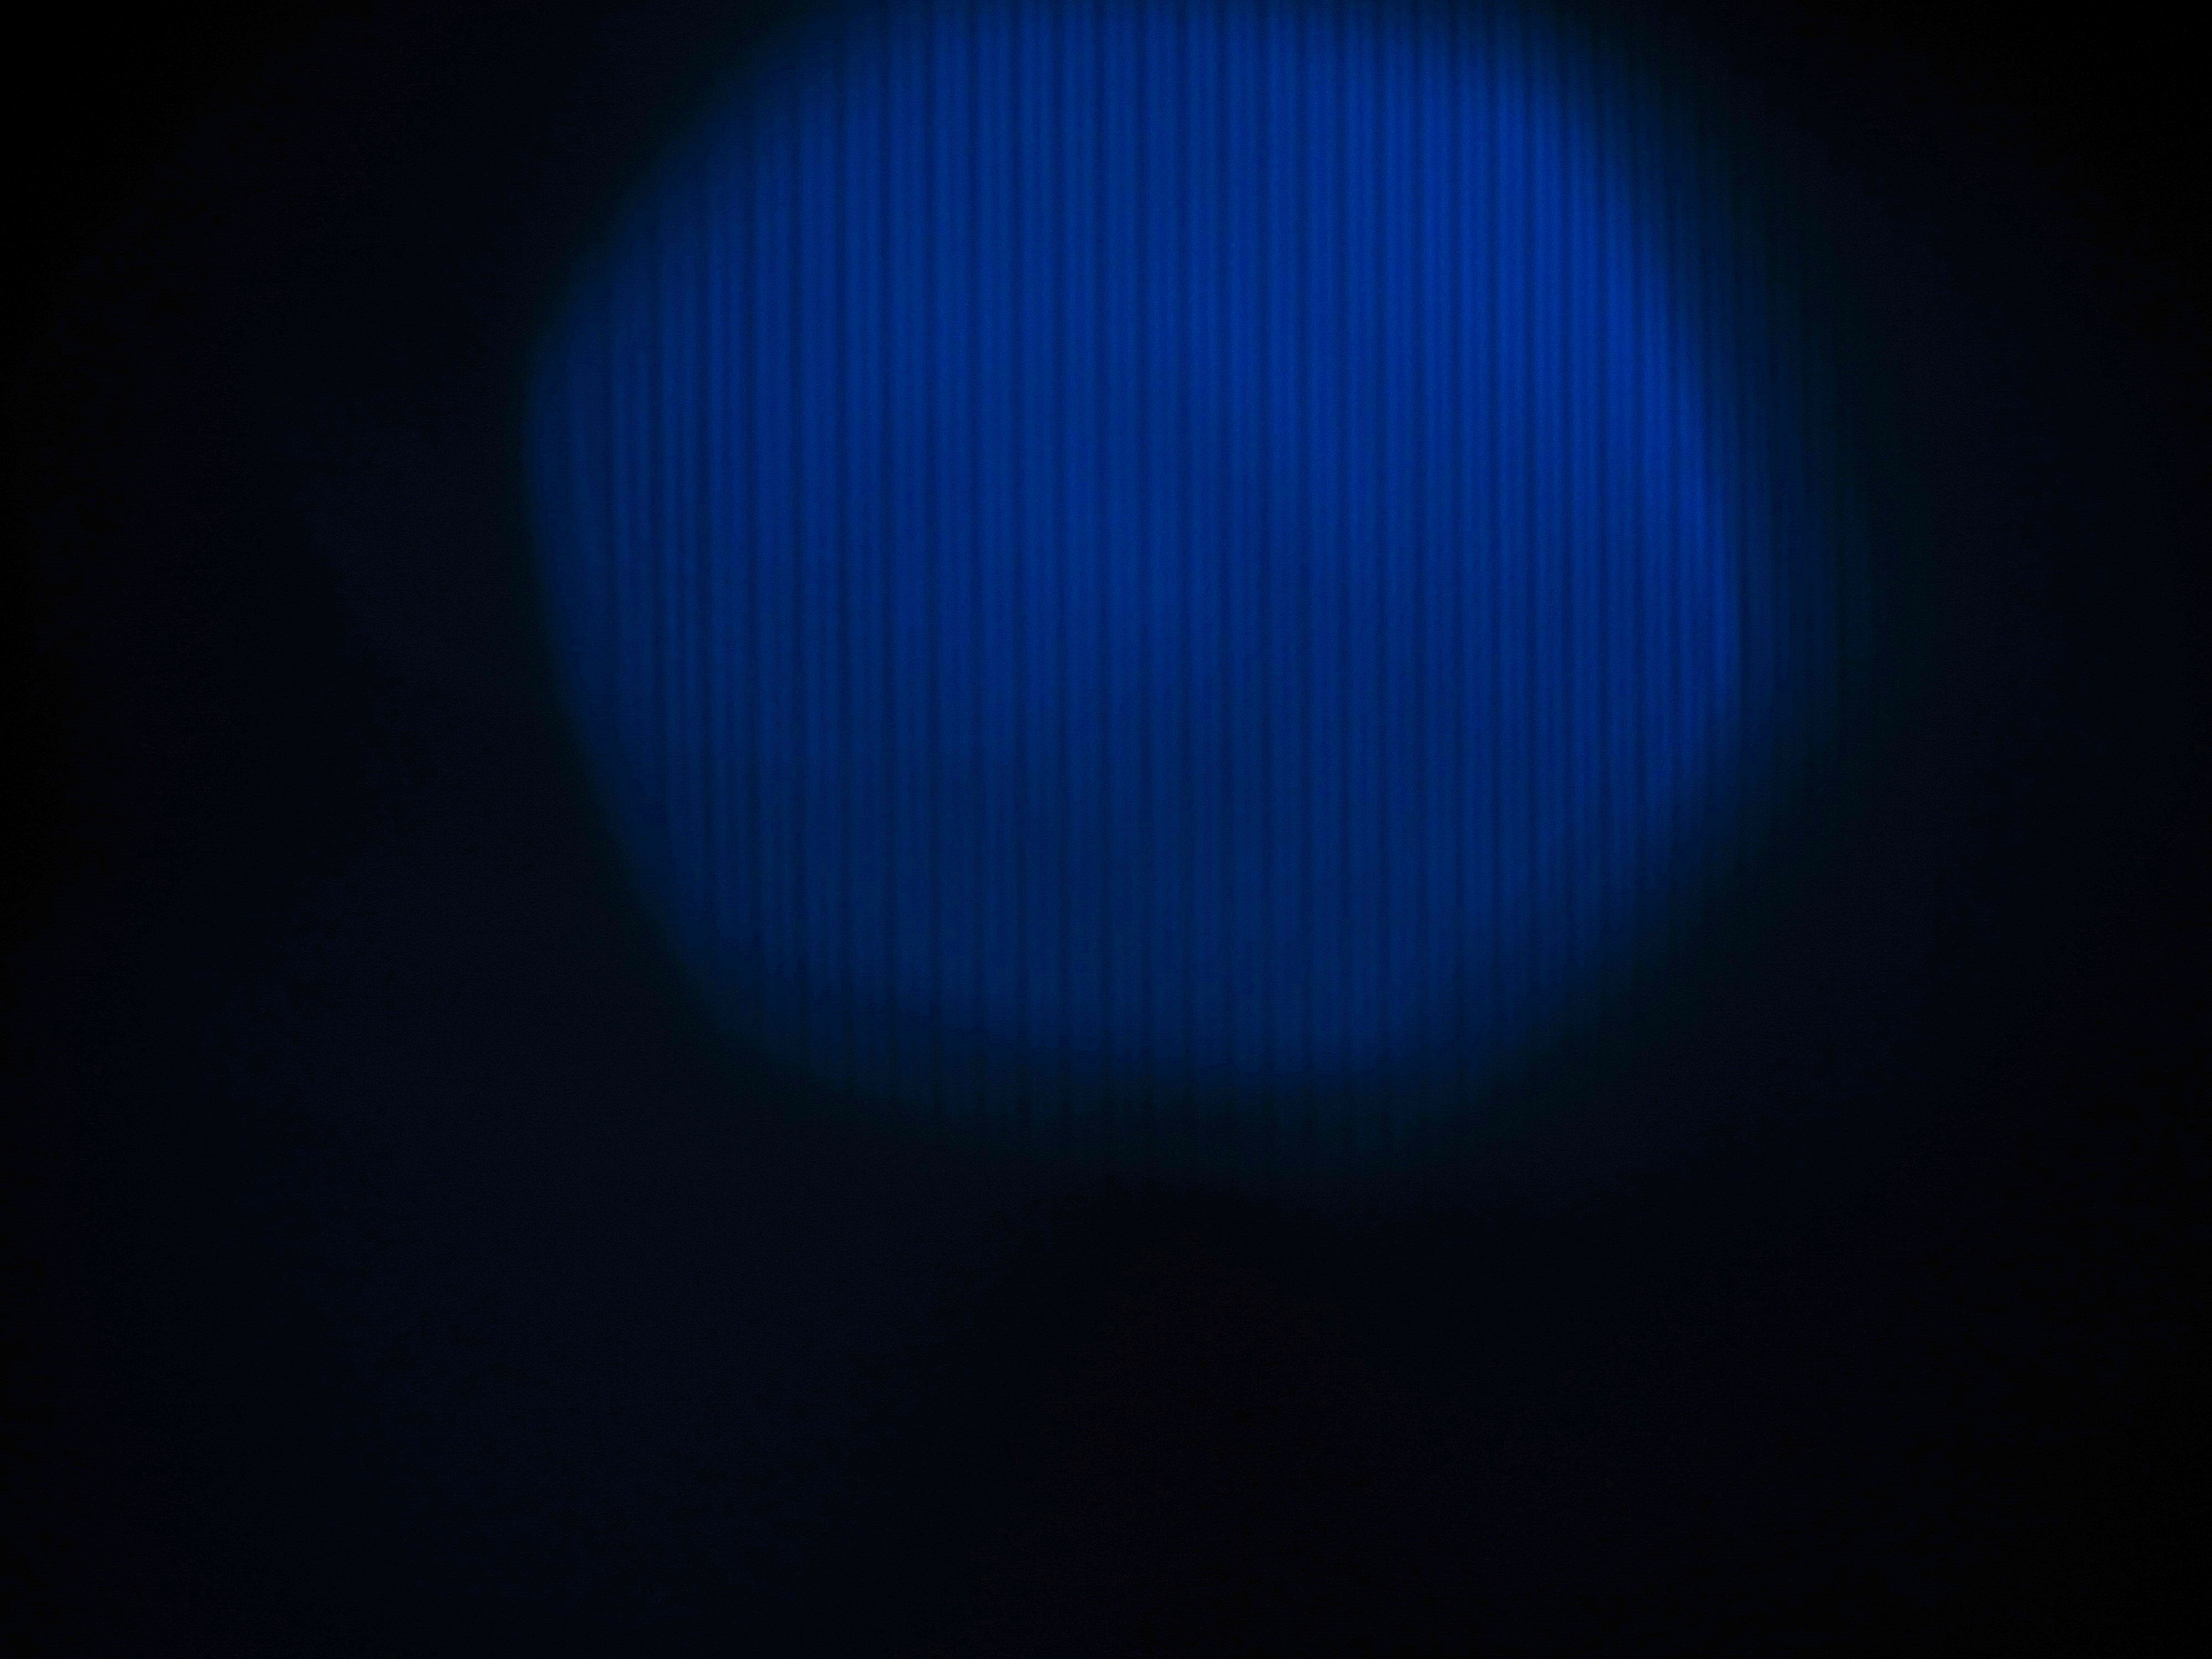
\includegraphics[width=0.45\textwidth]{IMG_0122k.jpg}
  \caption{Interferenzmuster der blauen Spektrallinie mit linear polarisiertem Licht mit Magnetfeld (nachbearbeitet).}
  \label{fig:b2}
\end{figure}
\FloatBarrier
\begin{figure}
  \centering
  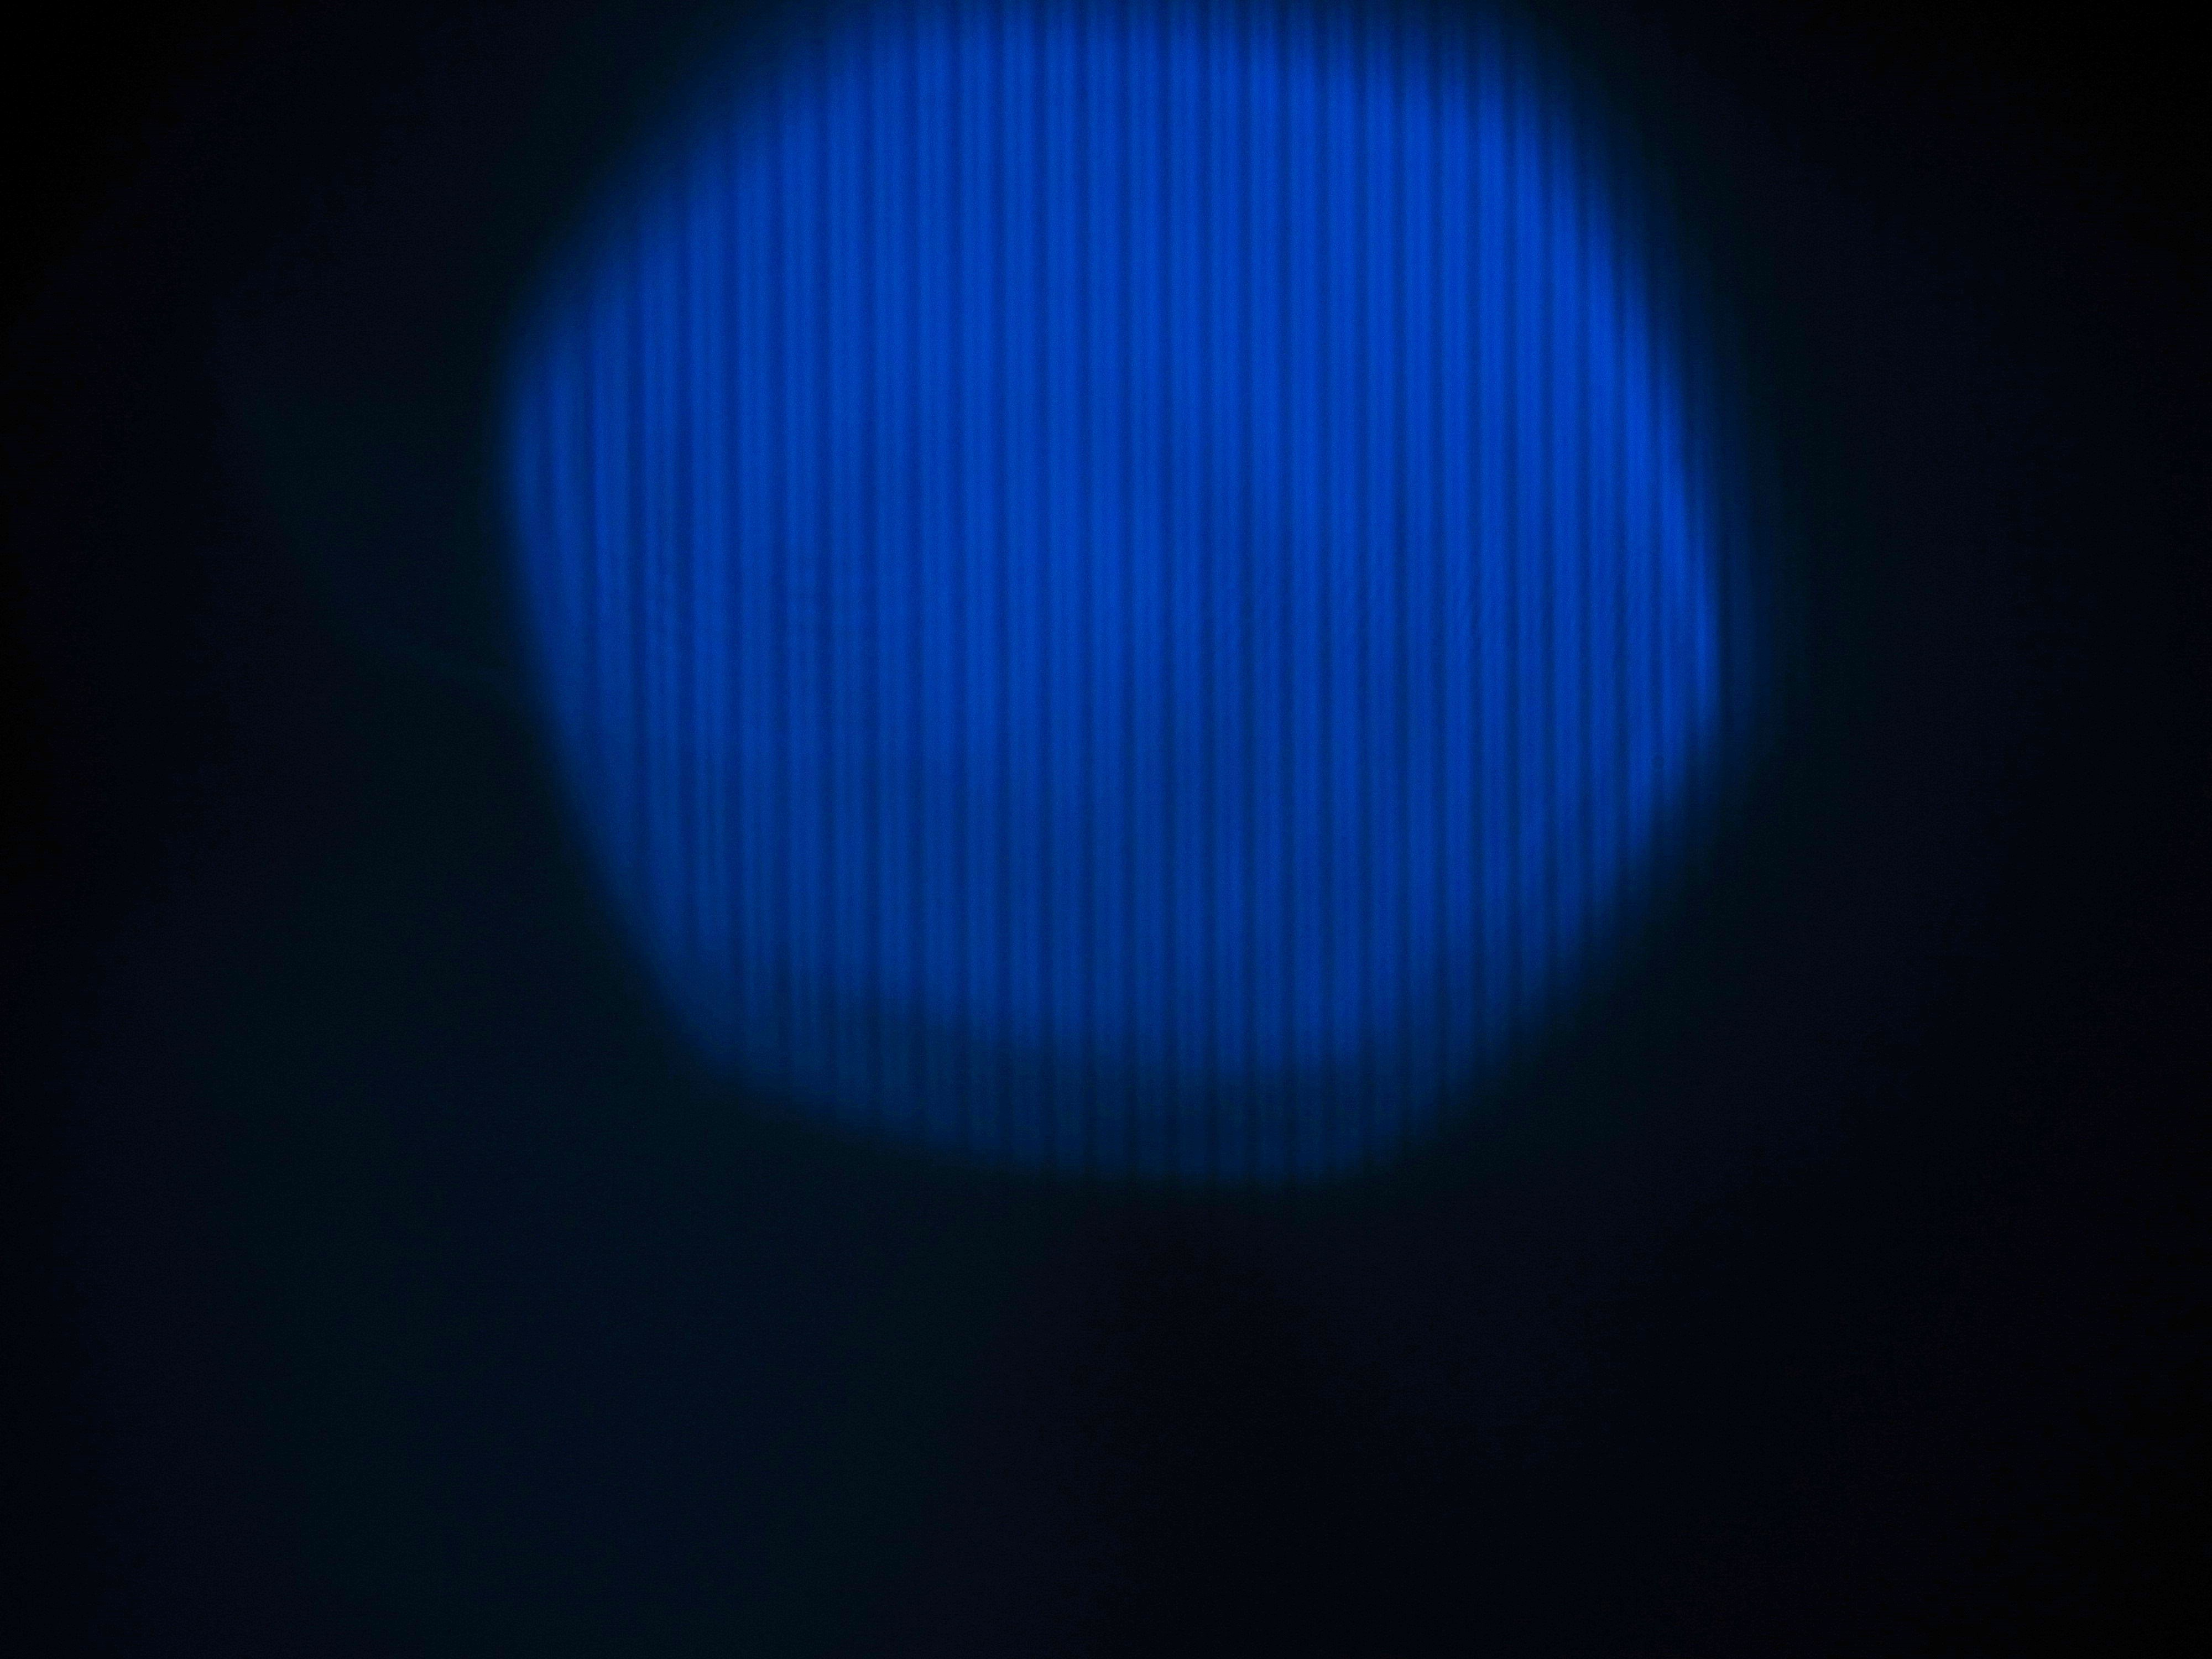
\includegraphics[width=0.45\textwidth]{IMG_0123k.jpg}
  \caption{Interferenzmuster der roten Spektrallinie mit zirkular polarisiertem Licht mit Magnetfeld (nachbearbeitet).}
  \label{fig:b3}
\end{figure}
\FloatBarrier

Die gemessenen Abstände und die mit \ref{eqn:} % 
berechneten Wellenlängenunterschiede sind in Tabelle \ref{tab:b} eingetragen. Weiter außen liegende Maxima werden nicht miteinbezogen,
da sie zu schlecht zu erkennen sind.
\FloatBarrier
\begin{table}
    \centering
    \caption{Magnetfeldstärke in Abhängigkeit von der Stromstärke.}
    \label{tab:b}
    \sisetup{table-format=2.2}
    \begin{tabular}{S[table-format=2.0] S[table-format=2.0] S[table-format=2.0] S[table-format=2.2] S[table-format=2.2] }
      \toprule
      %{$D$/cm}& \multicolumn{5}{c}{$U_{\symup{B}i} = \,\si{V}$}\\ überschrift über mehrere spalten
      %\midrule
      {$\increment s_{\si{b}}/\text{Pixel}$} & {$\delta s_{\text{b,\,}\sigma}\text{Pixel}$} & {$\delta s_{\text{b,\,}\pi}\text{Pixel}$} & {$\increment \lambda_{\text{b,\,}\sigma}/\text{pm}$} & {$\increment \lambda_{\text{b,\,}\pi}/\text{pm}$}\\
      \midrule
      \midrule
      84 & 37 & 37 & 10,77 & 10,77 \\
      85 & 42 & 39 & 12,08 & 11,22 \\
      87 & 36 & 31 & 10,12 &  8,71 \\
      84 & 42 & 35 & 12,23 & 10,19 \\
      80 & 40 & 33 & 12,23 & 10,09 \\
      83 & 33 & 33 &  9,72 &  9,72 \\
      79 & 35 & 30 & 10,83 &  9,28 \\
      77 & 33 & 28 & 10,48 &  8,89 \\
      73 & 25 & 38 &  8,37 & 12,73 \\
      80 & 37 & 29 & 11,31 &  8,86 \\
      78 & 27 & 30 &  8,46 &  9,40 \\
      74 & 33 & 28 & 10,90 &  9,25 \\
      71 & 28 & 27 &  9,64 &  9,30 \\
      76 & 28 & 31 &  9,01 &  9,97 \\
      69 & 31 & 31 & 10,98 & 10,98 \\
      73 & 32 & 30 & 10,72 & 10,05 \\
      67 & 31 & 26 & 11,31 &  9,49 \\
      71 & 28 & 28 &  9,64 &  9,64 \\
      69 & 25 & 27 &  8,86 &  9,57 \\
      67 & 33 & 28 & 12,04 & 10,22 \\
      66 & 30 & 22 & 11,11 &  8,15 \\
      70 & 33 & 23 & 11,53 &  8,03 \\
      65 & 28 & 26 & 10,53 &  9,78 \\
      64 & 31 & 25 & 11,84 &  9,55 \\
      67 & 29 & 26 & 10,58 &  9,49 \\
      63 & 26 & 23 & 10,09 &  8,93 \\
      63 & 31 & 23 & 12,03 &  8,93 \\
      \bottomrule
    \end{tabular}
\end{table}
\FloatBarrier

Die mit Formel \ref{eqn:X} und \ref{eqn:dX} bestimmten Mittelwerte sind 
\begin{align*}
  \increment \lambda_{\text{b,\,}\sigma} &= \SI{10.65\pm0.22}{\pico\meter}, \\
  \increment \lambda_{\text{b,\,}\pi} &= \SI{9.67\pm0.19}{\pico\meter}.
\end{align*}

  
  
  
 
 
 

 
 
 

 
 
 

 
 
 

 
 
 

 
 
 


 



  
  
 
  
  
  
 
  
  
  
 
  
  
  
 
  
  
  
 
  
  
 
